\subsection{Visualizing alignments with \prog{ssu-draw}}

Because SSU rRNA is about 1500 nt, SSU alignments of even a few
sequences are difficult to view in a meaningful way, and this is
especially true if the alignments contain thousands of sequences.
The \prog{ssu-draw} program can be used to generate secondary
structure diagrams for displaying alignment statistics, such as
location and frequency of insertions and deletions, as well as
individual aligned sequences. \prog{ssu-draw} can only be used for
alignments created using the three default models; it cannot
be used for alignments to models created using \prog{ssu-build}.
To draw alignment statistic diagrams of our \prog{myseqs} example
dataset, do:

\user{ssu-draw myseqs}




The \prog{esl-ssudraw} program introduced for visualizing masks
earlier in this tutorial can be also used to display statistics of
a particular alignment on the consensus SSU secondary structure of the
model used to create the alignment. As just shown in the previous example,
using \prog{esl-ssudraw} requires a template postscript file of the
consensus secondary structure. The template files for the 3 default
\textsc{ssu-align} version 0.1 seed models are included as
\prog{ssu-align-0.1/seeds/ss-diagrams/\{archaea,bacteria,eukarya\}-0p1.ps}. 
(Unfortunately, it is difficult to create new template files for
additional models you might build for your own analyses.) 

\prog{esl-ssudraw} can be run in two different modes. In the default
mode, \emph{alignment} mode, the structure diagrams will display
statistics on the alignment. In \emph{individual} mode, the structure
diagrams will show individual sequences in the alignment by displaying
the actual residues at each consensus position of the alignment. Note
that the diagrams always depict the consensus model defined in the
template file. In alignment mode, only statistics of consensus
positions are displayed. In individual mode, only residues that align to
consensus positions are displayed.

\subsubsection{Relevant options for alignment mode}

The following table summarizes the different statistics that can be
created by \prog{esl-ssudraw} in alignment mode.
The postscript and pdf files for each of
these diagrams for the archaea, bacteria and eukarya seeds
are included in  \prog{ssu-align-0.1/seeds/ss-diagrams/}, named as
indicated  in the ``file'' column of the table (with \prog{<fam>}
standing for \prog{archaea}, \prog{bacteria}, or \prog{eukarya}). 
Section~\ref{section:chap9} includes examples of some of these
figures for each seed, as indicated by the figure numbers in 
the ``figure'' column. 

\begin{center}
\begin{tabular}{llll} \hline
\prog{esl-ssudraw} option(s) & statistic                     &  figure & file \\ \hline
\prog{<none>}                & information content           & \ref{fig:eukinfo} & \prog{<fam>-0p1-info} \\
& & & \\
\prog{-q --prob}                & average posterior probability & none & \prog{<fam>-0p1-prob} \\
& & & \\
\prog{-q --ins}                 & frequency of insertions       & \ref{fig:eukins}   & \prog{<fam>-0p1-ins} \\
                             & after each position           & & \\
& & & \\
\prog{-q --dall}                & frequency of deletions        & \ref{fig:eukdel}  & \prog{<fam>-0p1-dall} \\
& & & \\
\prog{-q --dint}                & frequency of internal deletions & none  & \prog{<fam>-0p1-dint} \\
                             & (excluding terminal deletions)  & & \\
& & & \\
\prog{-q --struct}              & additional information from     & \ref{fig:euksinfo} & \prog{<fam>-0p1-struct} \\
                             & conserved structure \\
\end{tabular}
\end{center}

If more than one of these options are used, the program will create a
multi-page postscript document with each diagram on a separate page.
If the \prog{-q} option is omitted, the program will create the
information content diagram as the first page by default.
As an example of how these files were created, the command

\scriptuser{esl-ssudraw -q --dall ../eukarya-0p1.stk eukarya-0p1.ps eukarya-0p1-dall.ps}

was used to create Figure~\ref{fig:eukdel} while in the 
\prog{ssu-align-0.1/seeds/ss-diagrams/} directory.
The shell script
\prog{ssu-align-0.1/seeds/ss-diagrams/draw-ss-diagrams.sh}
was used to create all of these diagrams.

\subsubsection{Displaying masks and alignment statistics simultaneously}

The \prog{--mask} option can be used in combination with any of the
options listed in the above table to create diagrams 
with positions that are excluded from a mask appearing as open
circles. Figure~\ref{fig:bacdelmask} in section~\ref{section:chap9}
shows an example. That figure was created from the
\prog{ssu-align-0.1/seeds/ss-diagrams/} directory using the command:

\user{esl-ssudraw --mask ../bacteria-0p1-seed-realn.mask -q --dall \\
  ../bacteria-0p1.stk bacteria-0p1.ps bacteria-0p1-dall-wmask.ps}

The \prog{bacteria-0p1-seed-realn.mask} was created by realigning all
of the bacterial seed sequences in
\prog{ssu-align-0.1/seeds/bacteria-0p1.fa} to the default bacterial
CM, and using the default masking strategy outlined above 
(\prog{esl-alimanip --pfract 0.95 --pthresh 0.95})
on the resulting alignment. Analogous masks for archaea and eukarya
are included in the \prog{ssu-align-0.1/seeds/} directory, and PDF and
postscript files showing each of the masks on each of the diagrams
from the above table are included in 
\prog{ssu-align-0.1/seeds/ss-diagrams/}. The naming convention for
these diagrams is the same as indicated in the ``file'' column of the
above table, but with the suffix \prog{-wmask} appended.

\subsubsection{Displaying individual aligned sequences}

The \prog{--indi} option makes \prog{esl-ssudraw} run in individual
mode. When used by itself, the program will create a single page
postscript of the consensus sequence of the model. This is the
single sequence that the model most closely represents, and is the
highest scoring possible sequence to the model. In the diagram of the
consensus sequence, uppercase residues indicate highly conserved positions,
and lowercase residues indicate less well-conserved positions.

When the \prog{--indi} option is used together with \prog{--all}, the
resulting postscript file will have $N+1$ pages, one for each of the
$N$ sequences in the alignment, displaying the residue that sequence
contains at each consensus position of the alignment (gaps are
indicated by \prog{-} characters). The $+1$ is due to the first page,
which again displays the consensus sequence. This page is omitted if
the \prog{-q} option is also used.

When the \prog{--prob} option is used with \prog{--indi} and
\prog{--all}, there will be $2N+1$ (or $2N$ if {\prog -q} is used)
pages created. The $N$ additional pages will display the posterior
probability (alignment confidence estimate) of each aligned residue
for each of the $N$ sequences.

The next two pages include two diagrams from the postscript file 
\prog{bacteria-0p1-indi-all.ps} created with:

\user{esl-ssudraw -q --all --indi --prob ../bacteria-0p1.p.stk \\ bacteria-0p1.ps bacteria-0p1-indi-all.ps}

Again from the \prog{ssu-align-0.1/seeds/ss-diagrams/} directory.
The two diagrams included here correspond to the
\emph{Escherichia coli} sequence (\db{genbank} accession J01695) that
is commonly used as a reference SSU sequence. The first diagram shows
the sequence as it aligns to the default bacterial model and the
second diagram shows the posterior probabilities of that alignment.

\begin{figure}
\begin{center}
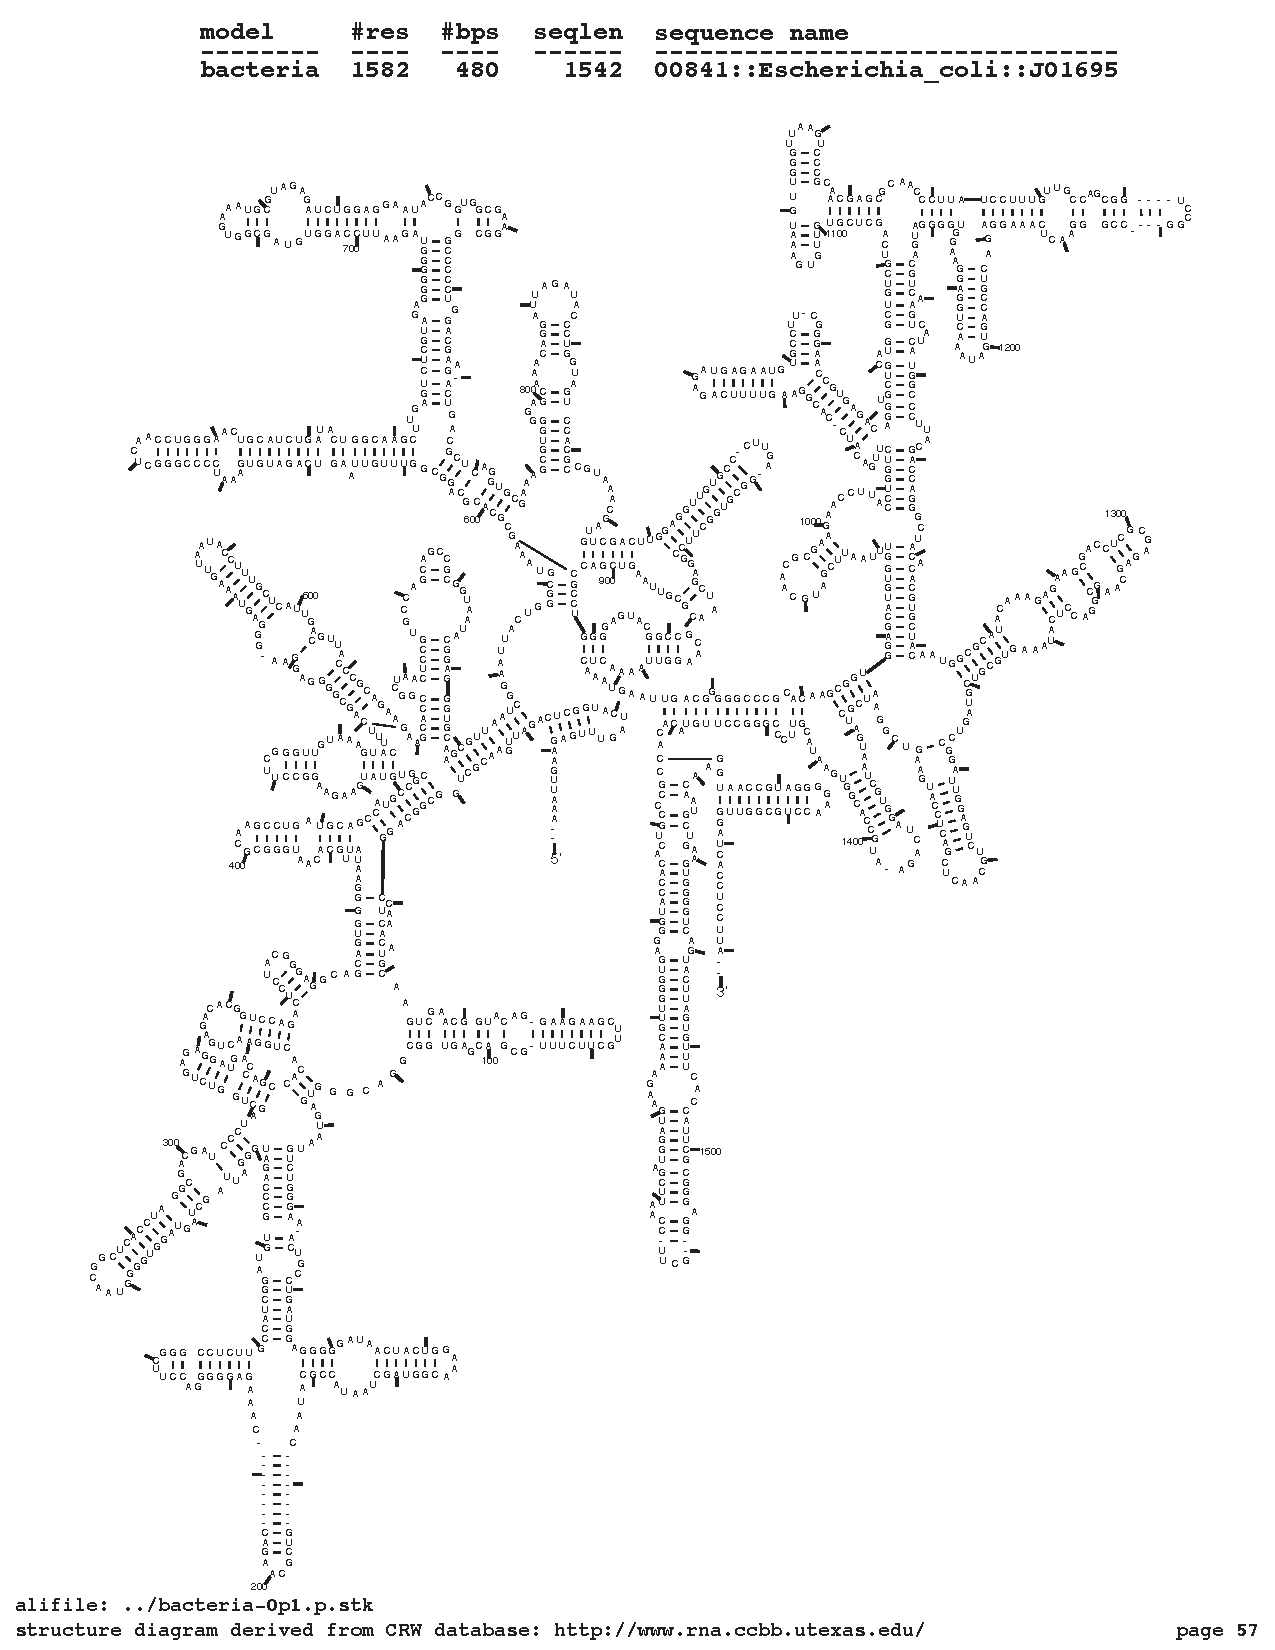
\includegraphics[width=5.7in]{Figures/ecoli-seq}
\end{center}
\caption{\textbf{The E. coli J01695 sequence aligned to the bacterial
SSU model.}}
\label{fig:ecoli-seq}
\end{figure}

\begin{figure}
\begin{center}
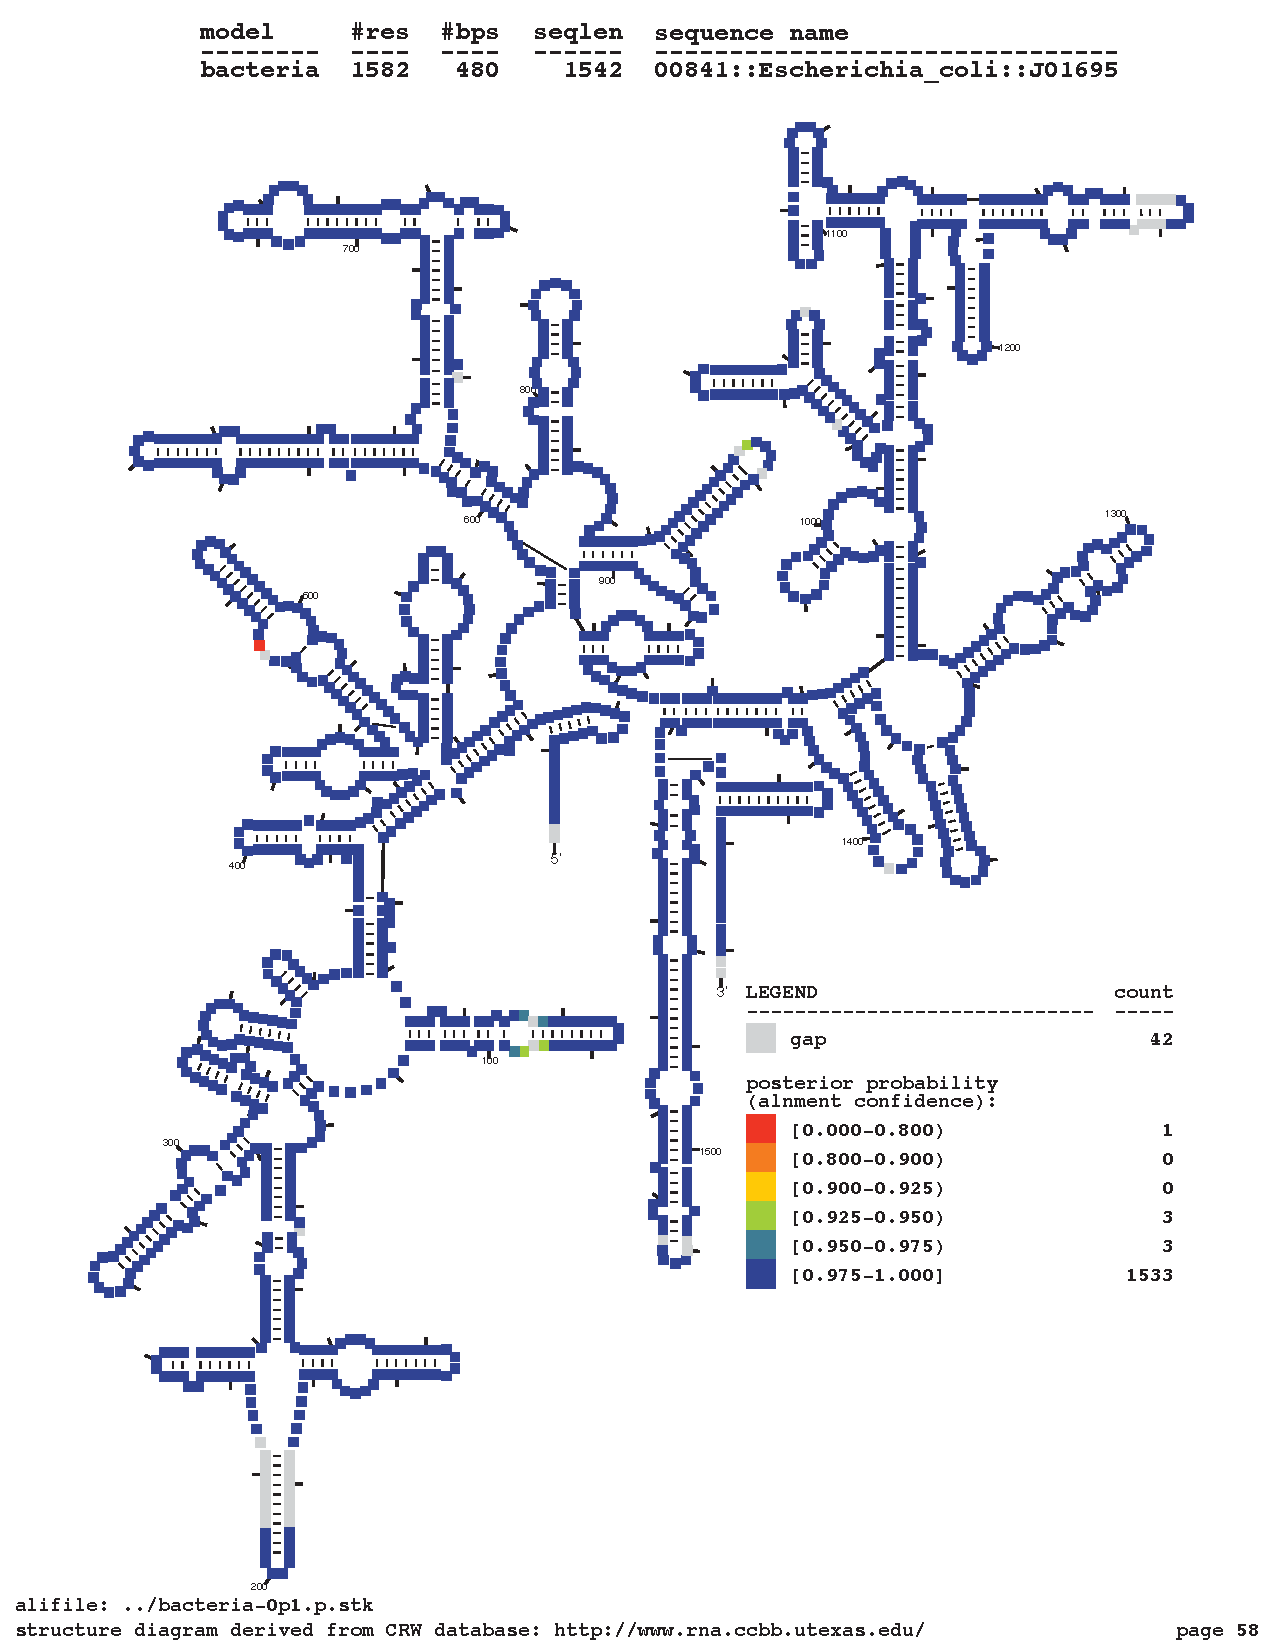
\includegraphics[width=5.7in]{Figures/ecoli-prob}
\end{center}
\caption{\textbf{The posterior probabilities of the aligned E. coli
J01695 sequence to the bacterial SSU model.}}
\label{fig:ecoli-prob}
\end{figure}




